% Chapter 3

\chapter{Methodology} % Methodology

\label{Chapter3} % For referencing the chapter elsewhere, use \ref{Chapter3} 

The research set out to evaluate different methods for estimating when a listening event is likely to occur. These were:

* Bayesian Counting
* Logistic Regression
* SVM
* Gaussian Processes
* Recurrent Neural Networks

The methodology employed is typical of that within the data science community, and as seen in online Kaggle competitions. Namely to start with preliminary analysis that will help understand the data better, then devise a test and training datasets that can be used across multiple models, with the main performance criteria being on how well the models perform on test data.

Python, via Jupyter notebooks was the primary source of analysis with some SQL as the data was manipualated and stored in a SqlLite3 database first.

Note: In the interest of time, analysis was carried out on 381 of the full 1000 user dataset.

\section{Preliminary analysis}

\subsection{Context}

Let us first consider the real-world aspect of the data we have - the timestamps on which users played a song. This does not necessarily mean they played the song in its entirety. Indeed initial analysis shows plenty of cases where a song was started, seconds after the previous one, suggesting that the dataset contains both tracks that were played and tracks that were skipped. For our purposes we can consider both these to be the same as they both indicate that the user was interested in playing music at time $t$.

We can also assume that the song plays are not i.i.d, in that the probability of a play event at time t+1 is significantly higher if there was an event at time t. 

\subsection{Basic statistics} 

We start with some basic information about the raw data file that was recieved. 
Num. of rows: 7,500,000
Num. of users: 381
Num. of unique timestamps: 7,226,934
earliest timestamp: 2005-02-14 00:02:10
latest timestamp: 2009-06-19 17:37:23

What does this tell us? Well we can deduce there are approximately 19.6k timestamps per user on average. This feels like a high number. Fig \ref{fig:fig1}

\begin{figure}[h!]
	\centering
	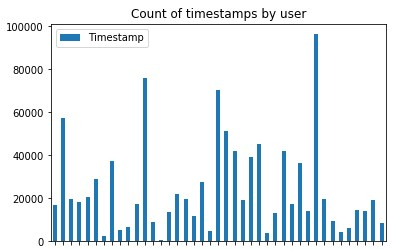
\includegraphics[width=7cm, keepaspectratio,]{fig002.jpg}
	\caption{}
	\label{fig:fig2}
\end{figure} 


\subsection{Outlier analysis} 


\section{Bayesian Inference}

Here we apply a counting process


\section{How to cite references in Latex}
\parencite{Reference1}

\medskip

This document is an example of \texttt{thebibliography} environment using 
in bibliography management. Three items are cited: \textit{The \LaTeX\ Companion} 
book \cite{latexcompanion}, the Einstein journal paper \cite{einstein}, and the 
Donald Knuth's website \cite{knuthwebsite}. The \LaTeX\ related items are
\cite{latexcompanion,knuthwebsite}. 

\medskip
